\documentclass[11pt]{book}
\usepackage{fontspec}
\setmainfont{TeX Gyre Pagella}
\usepackage[margin=1in]{geometry}
\usepackage{xcolor}
\usepackage{tikz}
\usetikzlibrary{arrows.meta,shapes.geometric,shapes.misc}
\usepackage{amssymb}
\usepackage{enumitem}
\usepackage{titlesec}

\titleformat{\chapter}[display]{\bfseries\Large}{Sproll 05}{0.5em}{\Huge}
\titleformat{\section}{\bfseries\large}{\thesection}{0.6em}{}

\newenvironment{algorithmproc}[1]{\vspace{0.6em}\noindent\rule{\linewidth}{0.6pt}\\[0.2em]\textbf{How to Tell: #1}\\[0.3em]}{\\[0.2em]\noindent\rule{\linewidth}{0.6pt}\vspace{0.6em}}
\newenvironment{practicenow}{\vspace{0.6em}\noindent\rule{\linewidth}{0.6pt}\\[0.2em]\textbf{Practice Now}\\[0.3em]}{\\[0.2em]\noindent\rule{\linewidth}{0.6pt}\vspace{0.6em}}
\newenvironment{exercisebox}[1]{\vspace{0.8em}\noindent\rule{\linewidth}{0.6pt}\\[0.2em]\textbf{Exercises: #1}\\[0.3em]\begin{enumerate}[label=\arabic*., itemsep=0.4em]}{\end{enumerate}\noindent\rule{\linewidth}{0.6pt}\vspace{0.6em}}
\newenvironment{trythis}{\vspace{0.6em}\noindent\rule{\linewidth}{0.6pt}\\[0.2em]\textbf{Try This}\\[0.3em]}{\\[0.2em]\noindent\rule{\linewidth}{0.6pt}\vspace{0.6em}}
\newenvironment{summarybox}{\vspace{0.6em}\noindent\rule{\linewidth}{0.6pt}\\[0.2em]\textbf{What We Learned}\\[0.3em]}{\\[0.2em]\noindent\rule{\linewidth}{0.6pt}\vspace{0.6em}}

\begin{document}
\begin{titlepage}
\centering
\vspace*{1.4in}
{\Huge \textbf{SPROLL 05}}\\[0.5in]
{\huge Together}\\[0.8in]
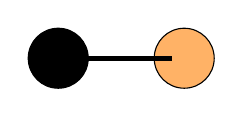
\begin{tikzpicture}
\filldraw[fill=black] (-0.8,0) circle (0.15in);
\filldraw[fill=orange!60] (0.8,0) circle (0.15in);
\draw[line width=1.8pt] (-0.65,0) -- (0.65,0);
\end{tikzpicture}\\[0.8in]
{\Large The Sproll Curriculum}\\[0.2in]
{\large Cycle I: Pops --- Things, Differences, and Counting}
\end{titlepage}

\tableofcontents

\chapter*{Before You Begin}
\addcontentsline{toc}{chapter}{Before You Begin}

So far, every Pop and every Refuse in this curriculum has stood alone. This workbook introduces the first way of connecting two things to each other on purpose, without making them into one thing. That distinction, connected but not combined, turns out to be surprisingly easy to blur, and this workbook exists to keep it sharp.

\chapter{Connected, But Not the Same Thing}

\section{Two Cars, One Coupler}

Picture two train cars linked together by a coupler. Push or pull one car, and the other moves with it. In that sense, the two cars now behave as a pair rather than as two independent objects. But they are still, unmistakably, two separate cars. You could count them, one and two. You could paint them different colors. If the coupler were removed, each car would still exist on its own, exactly as before.

\begin{center}
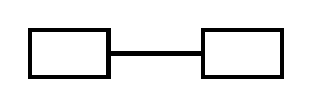
\begin{tikzpicture}
\draw[line width=1.5pt] (-1.6,-0.3) rectangle (-0.6,0.3);
\draw[line width=1.5pt] (0.6,-0.3) rectangle (1.6,0.3);
\draw[line width=2pt] (-0.6,0) -- (0.6,0);
\end{tikzpicture}
\end{center}

This curriculum calls this kind of deliberate connection a \textbf{Bind}. A Bind links two things so that something about one of them now depends on, or relates to, the other, without making the two things into a single thing. The two train cars are bound. They are not merged into one enormous car.

\begin{algorithmproc}{Is This a Bind?}
Ask two questions. First, are there still genuinely two separate things after the connection, each of which you could point to individually? Second, does something about them now depend on each other, so that moving or changing one has some effect on the other? If both answers are yes, you are looking at a Bind.
\end{algorithmproc}

\begin{practicenow}
Think of two objects in your life that are connected to each other on purpose, a leash and a collar, a key and a keyring, two socks kept as a pair. For each, confirm that both objects still exist separately even though they are connected.
\end{practicenow}

\begin{exercisebox}{Section 1.1}
\item Explain why two train cars connected by a coupler are still ``two cars'' rather than becoming ``one long car.''
\item Describe a connection in your own life where moving one connected object clearly causes an effect on the other.
\item Challenge: can two things be bound to each other without either one visibly moving when the other moves? Try to think of an example.
\end{exercisebox}

\chapter{Together Is Not Merged}

\section{Puzzle Pieces Versus Melted Candles}

Two puzzle pieces snapped together are bound: they now fit and move as a pair, but you can still see the seam between them, and you could pull them apart again. Compare this to two candles melted together in a fire. Once melted, there is no longer a seam, no way to point to ``this part was candle one'' and ``this part was candle two.'' The wax has become one single thing.

\begin{center}
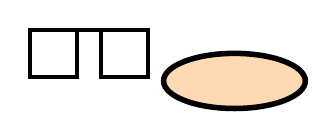
\begin{tikzpicture}
\draw[line width=1.5pt] (-1.8,-0.3) -- (-1.2,-0.3) -- (-1.2,0.3) -- (-0.9,0.3) -- (-0.9,-0.3) -- (-0.3,-0.3) -- (-0.3,0.3) -- (-1.8,0.3) -- cycle;
\draw[line width=2pt, fill=orange!30] (0.8,-0.35) ellipse (0.9 and 0.35);
\end{tikzpicture}
\end{center}

Puzzle pieces are an example of a Bind. Melted candles are an example of something else entirely, a genuine merging into one, which this curriculum reserves for a different action altogether, called Collapse, introduced in the next workbook. Bind never does this. No matter how tightly two things are bound, a Bind keeps them separately identifiable.

\begin{algorithmproc}{Bind Versus Merge}
If you can still point to where one part ends and the other begins, you are looking at a bind, no matter how tightly connected the two parts seem. If that boundary has genuinely disappeared, so that there is no longer a meaningful way to separate the two original things, something stronger than a bind has happened.
\end{algorithmproc}

\begin{trythis}
Snap two Lego bricks or puzzle pieces together, and separately, mix two colors of paint or play-dough together until you cannot tell them apart. Compare the two results. In which case can you still identify each original piece? In which case can you not?
\end{trythis}

\begin{exercisebox}{Section 2.1}
\item List two more examples of things that are clearly bound (connected, but still separately identifiable) from your everyday life.
\item List two examples of things that have been merged rather than merely bound (the original parts are no longer separately identifiable).
\item Challenge: is a smoothie made from several fruits a case of binding or merging? Explain your reasoning.
\end{exercisebox}

\chapter{Why Keep Them Separate}

\section{The Usefulness of Not Merging}

It might seem like binding is just a weaker, less complete version of merging, but that is exactly backwards. Binding preserves something merging destroys: the ability to still treat the parts individually when you need to. A dog on a leash is bound to its owner, not merged with them, precisely because both the dog and the owner need to remain able to move somewhat independently, sit, turn, stop, while still being connected for safety. If a dog and its owner were somehow merged into one being, the leash would be pointless, but so would the dog's and the owner's separate abilities to walk, sit, or turn on their own.

\begin{summarybox}
A Bind connects two things so that something about them now depends on each other, without making them into one single thing. Puzzle pieces, train cars, and a leash and its wearer are all bound, not merged: you can always still point to each original part. Merging, which erases that boundary entirely, is a different and stronger action, taken up in the next workbook.
\end{summarybox}

\begin{exercisebox}{Section 3.1}
\item Explain, using the dog-and-leash example, why keeping two things separate while still connecting them can be more useful than merging them into one.
\item Describe a situation where you would want two things bound together rather than merged, and explain why merging them would cause a problem.
\item Challenge: can a single object be bound to more than one other object at the same time? Give an example if you can think of one.
\end{exercisebox}

\chapter*{Looking Ahead}
\addcontentsline{toc}{chapter}{Looking Ahead}

Every group of shapes or dots in this curriculum so far has, at some point, been looked at as a whole: ``here is what we have now.'' But how exactly do you decide what to count, or what to see, when you look at a group of bound and unbound things together? That question, and the fourth and final primitive action of this curriculum, are the subject of the next workbook, Sproll 06: Look Through a Rule.

\chapter*{For Parents and Teachers}
\addcontentsline{toc}{chapter}{For Parents and Teachers}

This workbook introduces Bind, the third of the four primitive actions this curriculum builds from. The central point, that binding couples two elements without identifying them, is stated and re-stated deliberately, because the natural intuition is to treat ``connected'' and ``combined'' as the same idea. Chapter 2's contrast between puzzle pieces and melted candles exists specifically to head off that conflation before Sproll 06 introduces Collapse, which is where a genuine merging or identification of bound elements can occur, under a specific, named rule, rather than automatically.

\end{document}
